% -*- coding: utf-8 -*-
%-------------------------designed by zcf--------------
\documentclass[UTF8,a4paper,10pt]{ctexart}
\usepackage[left=3.17cm, right=3.17cm, top=2.74cm, bottom=2.74cm]{geometry}
\usepackage{amsmath}
\usepackage{graphicx,subfig}
\usepackage{float}
\usepackage{cite}
\usepackage{caption}
\usepackage{enumerate}
\usepackage{booktabs} %表格
\usepackage{multirow}
\usepackage{pythonhighlight}
\newcommand{\tabincell}[2]{\begin{tabular}{@{}#1@{}}#2\end{tabular}}  %表格强制换行
%-------------------------字体设置--------------
\usepackage{times} 
\newcommand{\yihao}{\fontsize{26pt}{36pt}\selectfont}           % 一号, 1.4 倍行距
\newcommand{\erhao}{\fontsize{22pt}{28pt}\selectfont}          % 二号, 1.25倍行距
\newcommand{\xiaoer}{\fontsize{18pt}{18pt}\selectfont}          % 小二, 单倍行距
\newcommand{\sanhao}{\fontsize{16pt}{24pt}\selectfont}  %三号字
\newcommand{\xiaosan}{\fontsize{15pt}{22pt}\selectfont}        % 小三, 1.5倍行距
\newcommand{\sihao}{\fontsize{14pt}{21pt}\selectfont}            % 四号, 1.5 倍行距
\newcommand{\banxiaosi}{\fontsize{13pt}{19.5pt}\selectfont}    % 半小四, 1.5倍行距
\newcommand{\xiaosi}{\fontsize{12pt}{18pt}\selectfont}            % 小四, 1.5倍行距
\newcommand{\dawuhao}{\fontsize{11pt}{11pt}\selectfont}       % 大五号, 单倍行距
\newcommand{\wuhao}{\fontsize{10.5pt}{15.75pt}\selectfont}    % 五号, 单倍行距
%-------------------------章节名----------------
\usepackage{ctexcap} 
\CTEXsetup[name={,、},number={ \chinese{section}}]{section}
\CTEXsetup[name={(,)},number={\chinese{subsection}}]{subsection}
\CTEXsetup[name={,.},number={\arabic{subsubsection}}]{subsubsection}
%-------------------------页眉页脚--------------
\usepackage{fancyhdr}
\pagestyle{fancy}
\lhead{\kaishu \leftmark}
% \chead{}
\rhead{\kaishu 机器学习实验报告}%加粗\bfseries 
\lfoot{}
\cfoot{\thepage}
\rfoot{}
\renewcommand{\headrulewidth}{0.1pt}  
\renewcommand{\footrulewidth}{0pt}%去掉横线
\newcommand{\HRule}{\rule{\linewidth}{0.5mm}}%标题横线
\newcommand{\HRulegrossa}{\rule{\linewidth}{1.2mm}}
%-----------------------伪代码------------------
\usepackage{algorithm}  
\usepackage{algorithmicx}  
\usepackage{algpseudocode}  
\floatname{algorithm}{Algorithm}  
\renewcommand{\algorithmicrequire}{\textbf{Input:}}  
\renewcommand{\algorithmicensure}{\textbf{Output:}} 
\usepackage{lipsum}  
\makeatletter
\newenvironment{breakablealgorithm}
  {% \begin{breakablealgorithm}
  \begin{center}
     \refstepcounter{algorithm}% New algorithm
     \hrule height.8pt depth0pt \kern2pt% \@fs@pre for \@fs@ruled
     \renewcommand{\caption}[2][\relax]{% Make a new \caption
      {\raggedright\textbf{\ALG@name~\thealgorithm} ##2\par}%
      \ifx\relax##1\relax % #1 is \relax
         \addcontentsline{loa}{algorithm}{\protect\numberline{\thealgorithm}##2}%
      \else % #1 is not \relax
         \addcontentsline{loa}{algorithm}{\protect\numberline{\thealgorithm}##1}%
      \fi
      \kern2pt\hrule\kern2pt
     }
  }{% \end{breakablealgorithm}
     \kern2pt\hrule\relax% \@fs@post for \@fs@ruled
  \end{center}
  }
\makeatother
%------------------------代码-------------------
\usepackage{xcolor} 
\usepackage{listings} 
\lstset{ 
breaklines,%自动换行
basicstyle=\small,
escapeinside=``,
keywordstyle=\color{ blue!70} \bfseries,
commentstyle=\color{red!50!green!50!blue!50},% 
stringstyle=\ttfamily,% 
extendedchars=false,% 
linewidth=\textwidth,% 
numbers=left,% 
numberstyle=\tiny \color{blue!50},% 
frame=trbl% 
rulesepcolor= \color{ red!20!green!20!blue!20} 
}
%------------超链接----------
\usepackage[colorlinks,linkcolor=black,anchorcolor=blue]{hyperref}
%------------------------TODO-------------------
\usepackage{enumitem,amssymb}
\newlist{todolist}{itemize}{2}
\setlist[todolist]{label=$\square$}
% for check symbol 
\usepackage{pifont}
\newcommand{\cmark}{\ding{51}}%
\newcommand{\xmark}{\ding{55}}%
\newcommand{\done}{\rlap{$\square$}{\raisebox{2pt}{\large\hspace{1pt}\cmark}}\hspace{-2.5pt}}
\newcommand{\wontfix}{\rlap{$\square$}{\large\hspace{1pt}\xmark}}
%------------------------水印-------------------
\usepackage{tikz}
\usepackage{xcolor}
\usepackage{eso-pic}

\newcommand{\watermark}[3]{\AddToShipoutPictureBG{
\parbox[b][\paperheight]{\paperwidth}{
\vfill%
\centering%
\tikz[remember picture, overlay]%
  \node [rotate = #1, scale = #2] at (current page.center)%
    {\textcolor{gray!80!cyan!30!magenta!30}{#3}};
\vfill}}}



%———————————————————————————————————————————正文———————————————————————————————————————————————
%----------------------------------------------
\begin{document}
\begin{titlepage}
    \begin{center}
    
\includegraphics[width=0.8\textwidth]{NKU.png}\\[1cm]    
    \textsc{\Huge \kaishu{\textbf{南\ \ \ \ \ \ 开\ \ \ \ \ \ 大\ \ \ \ \ \ 学}} }\\[0.9cm]
    \textsc{\huge \kaishu{\textbf{计\ \ 算\ \ 机\ \ 学\ \ 院}}}\\[0.5cm]
    \textsc{\Large \textbf{机器学习实验报告}}\\[0.8cm]
    \HRule \\[0.9cm]
    { \LARGE \bfseries 实验四\ 决策树分类器}\\[0.4cm]
    \HRule \\[2.0cm]
    \centering
    \textsc{\LARGE \kaishu{姓名\ :\ 王泳鑫}}\\[0.5cm]
    \textsc{\LARGE \kaishu{学号\ :\ 1911479}}\\[0.5cm]
    \textsc{\LARGE \kaishu{年级\ :\ 2019级}}\\[0.5cm]
    \textsc{\LARGE \kaishu{专业\ :\ 计算机科学与技术}}\\[0.5cm]
    \textsc{\LARGE \kaishu{指导教师\ :\ 卫金茂}}\\[0.5cm]
    \vfill
    {\Large \today}
    \end{center}
\end{titlepage}
%-------------摘------要--------------
\newpage
\thispagestyle{empty}
\renewcommand{\abstractname}{\kaishu \sihao \textbf{摘要}}
    \begin{abstract}

        \noindent  %顶格
        \textbf{\\\ 关键字:层次聚类,Machine Learning , Deep Learning}\textbf{} \\\ \\\
    \end{abstract}
%----------------------------------------------------------------
\tableofcontents
%----------------------------------------------------------------
\newpage
\watermark{60}{10}{NKU}
\setcounter{page}{1}
%——————————————————————————————————————
\section{实验描述与要求}

基本要求:绘制聚类前后样本分布情况

\begin{enumerate}
    \item 基于 Watermelon-train1数据集(只有离散属性),构造ID3决策树;
    \item 基于构造的 ID3 决策树,对数据集 Watermelon-test1进行预测,输出分类精度;
\end{enumerate}

中级要求:
\begin{enumerate}
    \item 对数据集Watermelon-train2,构造C4.5或者CART决策树,要求可以处理连续型属性;
    \item 对测试集Watermelon-test2进行预测,输出分类精度;
\end{enumerate}
%----------------------------------------------------------------

\section{程序设计与代码实现}


\subsection{ID3算法决策树构建}

首先,ID3算法的核⼼思想应用信息增益准则作为标准,我们根据公式就可以实现计算信息熵,代码如下:

\begin{python}
# 计算信息熵
def calculate_entropy(y):
    log2 = math.log2
    unique_labels = np.unique(y)
    entropy = 0
    for label in unique_labels:
        count = len(y[y == label])
        p = count / len(y)
        entropy += -p * log2(p)
    return entropy
\end{python}

接下来,我们需要定义树的节点,代码如下:

\begin{python}
class DecisionNode():
    def __init__(self, feature_i=None, threshold=None,
                 value=None, true_branch=None, false_branch=None):
        self.feature_i = feature_i
        self.threshold = threshold
        self.value = value
        self.true_branch = true_branch
        self.false_branch = false_branch

\end{python}

然后要对特征进行划分,代码如下:

\begin{python}
    def divide_on_feature(X, feature_i, threshold):
    split_func = None
    if isinstance(threshold, int) or isinstance(threshold, float):
        split_func = lambda sample: sample[feature_i] >= threshold
    else:
        split_func = lambda sample: sample[feature_i] == threshold

    X_1 = np.array([sample for sample in X if split_func(sample)])
    X_2 = np.array([sample for sample in X if not split_func(sample)])

    return np.array([X_1, X_2])
\end{python}

接着,就是我们决策树的内容,代码如下:

\begin{python}
    class DecisionTree(object):
    def __init__(self, min_samples_split=2, min_impurity=1e-7,
                 max_depth=float("inf"), loss=None):
        self.root = None  #根节点
        self.min_samples_split = min_samples_split
        self.min_impurity = min_impurity
        self.max_depth = max_depth
        # 计算值 如果是分类问题就是信息增益,回归问题就基尼指数
        self._impurity_calculation = None
        self._leaf_value_calculation = None #计算叶子
        self.one_dim = None
        self.loss = loss

    def fit(self, X, y, loss=None):
        self.one_dim = len(np.shape(y)) == 1
        self.root = self._build_tree(X, y)
        self.loss=None

    def _build_tree(self, X, y, current_depth=0):
        """
        递归求解树
        """

        largest_impurity = 0
        best_criteria = None
        best_sets = None

        if len(np.shape(y)) == 1:
            y = np.expand_dims(y, axis=1)

        Xy = np.concatenate((X, y), axis=1)

        n_samples, n_features = np.shape(X)

        if n_samples >= self.min_samples_split and current_depth <= self.max_depth:
            # 计算每一个特征的增益值
            for feature_i in range(n_features):
                feature_values = np.expand_dims(X[:, feature_i], axis=1)
                unique_values = np.unique(feature_values)

                for threshold in unique_values:
                    Xy1, Xy2 = divide_on_feature(Xy, feature_i, threshold)

                    if len(Xy1) > 0 and len(Xy2) > 0:
                        y1 = Xy1[:, n_features:]
                        y2 = Xy2[:, n_features:]

                        # 计算增益值
                        impurity = self._impurity_calculation(y, y1, y2)

                        if impurity > largest_impurity:
                            largest_impurity = impurity
                            best_criteria = {"feature_i": feature_i, "threshold": threshold}
                            best_sets = {
                                "leftX": Xy1[:, :n_features],
                                "lefty": Xy1[:, n_features:],
                                "rightX": Xy2[:, :n_features],
                                "righty": Xy2[:, n_features:]
                            }

        if largest_impurity > self.min_impurity:
            true_branch = self._build_tree(best_sets["leftX"], best_sets["lefty"], current_depth + 1)
            false_branch = self._build_tree(best_sets["rightX"], best_sets["righty"], current_depth + 1)
            return DecisionNode(feature_i=best_criteria["feature_i"], threshold=best_criteria[
                "threshold"], true_branch=true_branch, false_branch=false_branch)

        # 计算节点的目标值
        leaf_value = self._leaf_value_calculation(y)

        return DecisionNode(value=leaf_value)


    def predict_value(self, x, tree=None):
        """
        预测
        """

        if tree is None:
            tree = self.root

        if tree.value is not None:
            return tree.value

        feature_value = x[tree.feature_i]

        branch = tree.false_branch
        if isinstance(feature_value, int) or isinstance(feature_value, float):
            if feature_value >= tree.threshold:
                branch = tree.true_branch
        elif feature_value == tree.threshold:
            branch = tree.true_branch

        return self.predict_value(x, branch)

    def predict(self, X):
        y_pred = []
        for x in X:
            y_pred.append(self.predict_value(x))
        return y_pred
\end{python}

最后是分类器的实现,代码如下:

\begin{python}
    class ClassificationTree(DecisionTree):
    def _calculate_information_gain(self, y, y1, y2):
        # 计算信息增益
        p = len(y1) / len(y)
        entropy = calculate_entropy(y)
        info_gain = entropy - p * calculate_entropy(y1) - (1 - p) * calculate_entropy(y2)

        return info_gain

    def _majority_vote(self, y):
        most_common = None
        max_count = 0
        for label in np.unique(y):
            # 投票决定当前的节点为哪一个类
            count = len(y[y == label])
            if count > max_count:
                most_common = label
                max_count = count

        return most_common

    def fit(self, X, y):
        self._impurity_calculation = self._calculate_information_gain
        self._leaf_value_calculation = self._majority_vote
        super(ClassificationTree, self).fit(X, y)

\end{python}

\subsection{CART决策树构建}

对于CART决策树,我们只需要把ID3算法中计算信息熵函数修改为计算基尼系数的函数,代码如下:

\begin{python}
    def calculate_variance(X):
    """ Return the variance of the features in dataset X """
    mean = np.ones(np.shape(X)) * X.mean(0)
    n_samples = np.shape(X)[0]
    variance = (1 / n_samples) * np.diag((X - mean).T.dot(X - mean))

    return variance

\end{python}

同时把分类器中计算函数修改为:

\begin{python}
    def _calculate_variance_reduction(self, y, y1, y2):
    var_tot = calculate_variance(y)
    var_1 = calculate_variance(y1)
    var_2 = calculate_variance(y2)
    frac_1 = len(y1) / len(y)
    frac_2 = len(y2) / len(y)

    # 使用方差缩减
    variance_reduction = var_tot - (frac_1 * var_1 + frac_2 * var_2)

    return sum(variance_reduction)
\end{python}


\section{测试与结果演示}

\subsection{ID3决策树}

通过测试数据集来测试,代码如下:

\begin{python}
from sklearn.metrics import accuracy_score

x_train = np.loadtxt('D:\\Data\\lab6\\Watermelon-train1.csv',dtype='str',delimiter=',',skiprows=1,usecols=(1,2,3,4))
y_train = np.loadtxt('D:\\Data\\lab6\\Watermelon-train1.csv',dtype='str',delimiter=',',skiprows=1,usecols=(5))

x_test = np.loadtxt('D:\\Data\\lab6\\Watermelon-test1.csv',dtype='str',delimiter=',',skiprows=1,usecols=(1,2,3,4))
y_test = np.loadtxt('D:\\Data\\lab6\\Watermelon-test1.csv',dtype='str',delimiter=',',skiprows=1,usecols=(5))

clf = ClassificationTree()
clf.fit(x_train,y_train)


y_pred = clf.predict(x_test)

accuracy = accuracy_score(y_pred,y_test)

print(accuracy)
\end{python}

结果如图\ref{fig:1}所示
\begin{figure}[H]
    \centering
    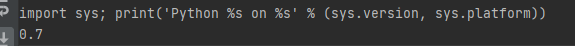
\includegraphics[scale=0.3]{1.png}
    \caption{ID3决策树结果}
    \label{fig:1}
\end{figure}

\subsection{CART决策树}

这里需要注意的是我们需要把密度从字符串形式转换为float类型,代码如下:

\begin{python}
from sklearn.metrics import accuracy_score

x_train = np.loadtxt('D:\\Data\\lab6\\Watermelon-train2.csv',dtype='str',delimiter=',',skiprows=1,usecols=(1,2,3,4,5))
y_train = np.loadtxt('D:\\Data\\lab6\\Watermelon-train2.csv',dtype='str',delimiter=',',skiprows=1,usecols=(6))

for i in range(17):
    x_train[i][4]=float(x_train[i][4])

x_test = np.loadtxt('D:\\Data\\lab6\\Watermelon-test2.csv',dtype='str',delimiter=',',skiprows=1,usecols=(1,2,3,4,5))
y_test = np.loadtxt('D:\\Data\\lab6\\Watermelon-test2.csv',dtype='str',delimiter=',',skiprows=1,usecols=(6))

for i in range(5):
    x_test[i][4]=float(x_train[i][4])

clf = RegressionTree()
clf.fit(x_train,y_train)


y_pred = clf.predict(x_test)

accuracy = accuracy_score(y_pred,y_test)

print(accuracy)
\end{python}


结果如图\ref{fig:1}所示
\begin{figure}[H]
    \centering
    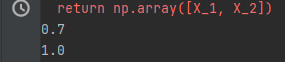
\includegraphics[scale=0.3]{2.png}
    \caption{CART决策树结果}
    \label{fig:1}
\end{figure}


%----------------------------------------------------------------
\bibliographystyle{plain}
\end{document}
